\documentclass{article} % Класс печатного документа

% для поддержки русского языка
\usepackage[T2A]{fontenc} % поддержка специальных русских символов
\usepackage[utf8]{inputenc} % Кодировка исходного текста - utf8
\usepackage[english,russian]{babel} % Поддержка языка - русского с английским
\usepackage{indentfirst} % Отступ в первом абзаце

\usepackage{graphicx} % Для вставки картинок
\usepackage{hyperref} % Для вставки гиперссылок
\usepackage{listings} % Для вставки кусков кода
\usepackage{float} % Для точного позиционирования картинок
\usepackage{amsmath} % Для отключения нумерации у указанных формул
\usepackage{listings} % Добавление листингов
\usepackage[justification=centering]{caption} % для центрирования подписи к таблице

\title{Отчёт 4\\
Определение достаточного количества факторов\\
факторного анализа} % заголовок документа
\author{Свичкарев А.\,В.} % Автор документа
\date{\today} % Текущая дата

\begin{document} % Конец преамбулы, начало текста

\maketitle % Печатает заголовок, список авторов и дату

\section*{Задачи}
Дана таблица корреляций 5 факторов.

На основе факторного анализа найти
достаточное количество факторов,
которого будет достаточно для
объяснения корреляции внутри набора наблюдаемых переменных
меньшим набором более фундаментальных ненаблюдаемых
переменных, которые лежат в основе данных.
\begin{table}[H]
\centering
\begin{tabular}{|c|c|c|c|c|c|}
\hline
        & Factor1 & Factor2 & Factor3 & Factor4 & Factor5\\ \hline
Factor1 & 1       & 0.02    & 0.96    & 0.42    & 0.01 \\ \hline
Factor2 & 0.02    & 1       & 0.13    & 0.71    & 0.85 \\ \hline
Factor3 & 0.96    & 0.13    & 1       & 0.5     & 0.11 \\ \hline
Factor4 & 0.42    & 0.71    & 0.5     & 1       & 0.79 \\ \hline
Factor5 & 0.01    & 0.85    & 0.11    & 0.79    & 1    \\ \hline
\end{tabular}
\caption{Исходная таблица корреляций}
\end{table}

\clearpage
\section*{Выполнение}
\begin{figure}[H]
    \centering
    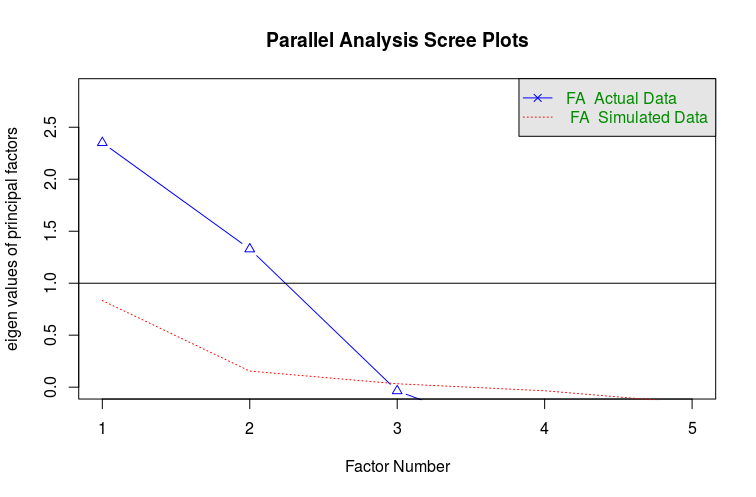
\includegraphics[width=\textwidth]{screeFa}
    \caption{Диаграмма каменистой осыпи с параллельным анализом
    для факторного анализа}
\end{figure}

В случае FA ясно видно, что нужно выделять два фактора.
Первые два собственных значения (треугольники) находятся выше изгиба
кривой собственных значений, а также превышают среднее значение
собственных значений, полученных на основании 100 симулированных матриц данных.
Для EFA собственные значения, согласно критерию Кайзера-Харриса, должны превышать 0.

Результат выделения двух общих факторов:

\begin{lstlisting}
Factor Analysis using method =  ml
Call: fa(r = corr, nfactors = 2, rotate = "none", fm = "ml")
Standardized loadings (pattern matrix) based upon correlation matrix
         ML1   ML2   h2    u2 com
Factor1 0.98 -0.14 0.97 0.028 1.0
Factor2 0.15  0.86 0.76 0.237 1.1
Factor3 0.98 -0.03 0.96 0.040 1.0
Factor4 0.54  0.74 0.83 0.168 1.8
Factor5 0.15  0.96 0.95 0.052 1.0

                       ML1  ML2
SS loadings           2.24 2.23
Proportion Var        0.45 0.45
Cumulative Var        0.45 0.89
Proportion Explained  0.50 0.50
Cumulative Proportion 0.50 1.00

Mean item complexity =  1.2
Test of the hypothesis that 2 factors are sufficient.

The degrees of freedom for the null model are  10  and the objective function was  5.6
The degrees of freedom for the model are 1  and the objective function was  0.02 

The root mean square of the residuals (RMSR) is  0 
The df corrected root mean square of the residuals is  0.01 

Fit based upon off diagonal values = 1
Measures of factor score adequacy             
                                                ML1  ML2
Correlation of scores with factors             0.99 0.98
Multiple R square of scores with factors       0.98 0.96
Minimum correlation of possible factor scores  0.97 0.92
\end{lstlisting}

Отсюда видно, что два фактора учитывают 89\%
дисперсии результатов 5 исходных признаков.

\section*{Вывод}
Для данной корреляционной матрицы разумно выделить два общих фактора.
Если говорить очень приблежённо,
то первый общий фактор будет отвечать
преимущественно из 1 и 3 исходных факторов,
второй общий фактор будет отвечать за 2, 3 и 5.

\section*{Исходный код}
Исходный код прилагается.

\end{document} % Конец документа
